\subsection*{Elementary Matrices}

\ul{Identity}
\iMbox{\mathbf{I}_{n} = [\mathbf{e}_{1}|\dots|\mathbf{e}_{n}] = [\mathbf{e}_{1};\dots;\mathbf{e}_{n}]}
has \ul{elementary vectors} \iMbox{\mathbf{e}_{1},\dots,\mathbf{e}_{n}}
for rows/columns

\textbf{Row/column switching}: \ul{permutation matrix} \iMbox{ P_{ij}}
obtained by \ul{switching} \iMbox{\mathbf{e}_{i}} and
\iMbox{\mathbf{e}_{j}} in \iMbox{\mathbf{I}_{n}} \emph{(same for rows/columns)}
\begin{itemize}

      \vItem
            Applying \iMbox{ P_{ij}} \textbf{from left} will \ul{swap rows},
            \textbf{from right} will \ul{swap columns}
      \vItem
            \iMbox{ P_{ij} = P_{ij}^{T} = P_{ij}^{-1}}, i.e. \ul{applying twice}
            will \textbf{undo} it
\end{itemize}

\textbf{Row/column scaling}: \iMbox{ D_{i}(\lambda)} obtained by \ul{scaling} \iMbox{\mathbf{e}_{i}} by \iMbox{\lambda} in
\iMbox{\mathbf{I}_{n}} \emph{(same for rows/columns)}
\begin{itemize}
      \vItem
            Applying \iMbox{ P_{ij}} \textbf{from left} will \ul{scale rows},
            \textbf{from right} will \ul{scale columns}
      \vItem
            \iMbox{ D_{i}(\lambda) = \mathrm{diag}(1,\dots,\lambda,\dots,1)}
            so all \textbf{diagonal} \ul{properties} apply,
            e.g. \iMbox{ D_{i}(\lambda)^{-1} = D_{i}(\lambda^{-1})}
\end{itemize}

\textbf{Row addition}:
\iMbox{ L_{ij}(\lambda) = \mathbf{I}_{n} + \lambda\mathbf{e}_{i}\mathbf{e}_{j}^{T}}
performs \iMbox{ R_{i} \leftarrow R_{i} + \lambda R_{j}} when
applying \textbf{from left}
\begin{itemize}

      \vItem
            \iMbox{\lambda\mathbf{e}_{i}\mathbf{e}_{j}^{T}} is \ul{zeros} except
            for \textbf{\iMbox{\lambda} in \iMbox{(i,j)}-th entry}
      \vItem
            \iMbox{L_{ij}(\lambda)^{-1} = L_{ij}(-\lambda)} both \ul{triangular matrices}
\end{itemize}


\subsection*{LU factorization w/ Gaussian elimination}

\ul{Recall:} you can represent \textbf{EROs} and
\textbf{ECOs} as \ul{transformation matrices} \iMbox{R,C}
\emph{respectively}

\textbf{\iMbox{LU} factorization} => finds \iMbox{A = LU}
where \iMbox{L,U} are \ul{lower/upper triangular} \emph{respectively}

\hSep % ---

\textbf{Naive Gaussian Elimination} performs
\iMbox{ [I_{m} \ | \ A \ | \ I_{n}] \rightsquigarrow [R^{-1} \ | \ U \ | \ I_{n}]}
to get \iMbox{AI_{n} = R^{-1}U} using \ul{only row addition}
\begin{itemize}
      \vItem
            \iMbox{R^{-1}}, i.e. \textbf{inverse EROs} in \ul{reversed order}, is
            \textbf{lower-triangular} so \iMbox{L = R^{-1}}

            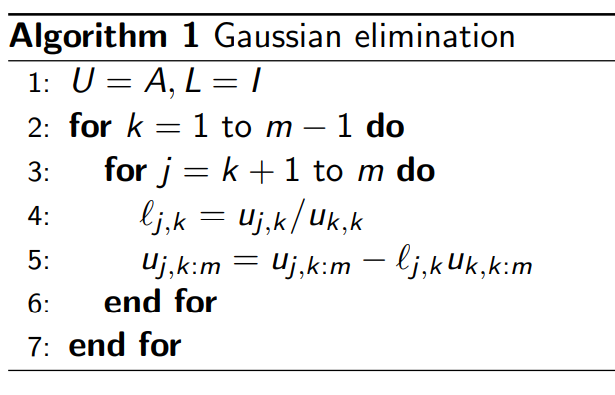
\includegraphics[width=75pt]{gausselim}
      \vItem
            The \textbf{pivot element} is simply \ul{diagonal entry}
            \iMbox{ u_{kk}^{(k-1)}}; fails if
            \iMbox{ u_{kk}^{(k-1)} \approx 0}
      \vItem
            \iMbox{\tilde{L} \tilde{U}=A+\delta A},
            \iMbox{ \frac{\|\delta A\|}{\|L\| \cdot\|U\|}= O\left(\epsilon_{ \mathrm{mach}}\right)};
            only \textbf{backwards stable} if
            \iMbox{\|L\| \cdot\|U\| \approx\|A\|}
      \vItem
            \ul{Work required:} \iMbox{{\sim}\frac{2}{3} m^3} flops
            \iMbox{{\sim}O\left(m^3\right)}
      \vItem
            Solving \iMbox{Ax = LUx} is \iMbox{{\sim}\frac{2}{3} m^3} flops
            \emph{(back substitution is \iMbox{O(m^2)})}
      \vItem
            \textbf{NOTE:} \ul{Householder triangularisation} requires
            \iMbox{{\sim}\frac{4}{3} m^3}
\end{itemize}

\hSep % ---

\textbf{Partial pivoting} computes \iMbox{PA = LU} where \iMbox{P} is
a \ul{permutation matrix} => \iMbox{PP^{T} = I}, i.e. its \ul{orthogonal}

\begin{itemize}

      \vItem
            For \ul{each column} \iMbox{j}, finds \ul{largest entry} and {row-swaps} to make
            it \ul{new pivot} => \iMbox{ P_{j}}
      \vItem
            Then performs \ul{normal elimination} on that column => \iMbox{ L_{j}}
      \vItem
            Result is \iMbox{ L_{m-1} P_{m-1} \ldots L_2 P_2 L_1 P_1 A = U},
            where \iMbox{ L_{m-1} P_{m-1} \ldots L_2 P_2 L_1 P_1=L_{m-1}^{\prime} \ldots L_1^{\prime} P_{m-1} \ldots P_1}
      \vItem
            Setting
            \iMbox{ L=\left(L_{m-1}^{\prime} \ldots L_1^{\prime}\right)^{-1}},
            \iMbox{ P=P_{m-1} \ldots P_1} gives \iMbox{P A=L U}

            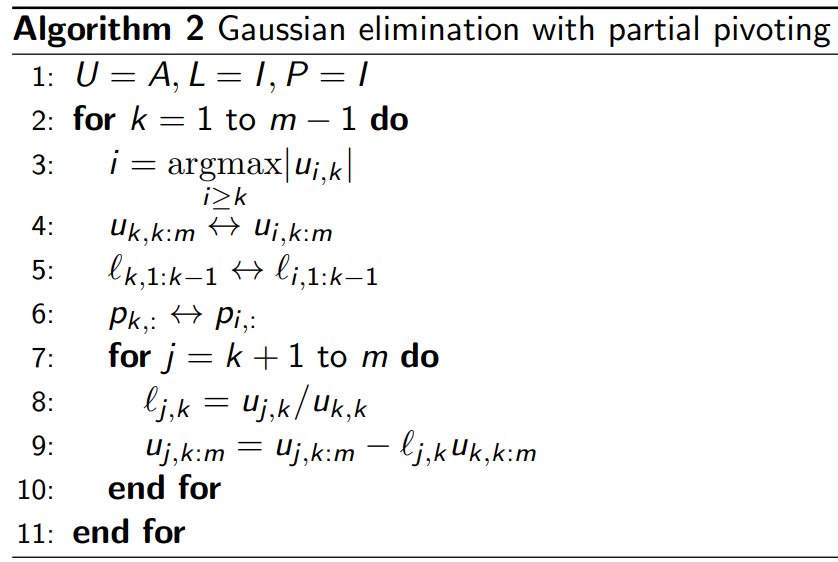
\includegraphics[width=100pt]{parpivot}
      \vItem
            \ul{Work required:} \iMbox{{\sim}\frac{2}{3} m^3} flops
            \iMbox{{\sim}O\left(m^3\right)}; results in \iMbox{ L_{ij} \leq 1} so \iMbox{ \lVert L \rVert = O(1)}
      \vItem
            \ul{Stability} depends on \textbf{growth-factor}
            \iMbox{\rho=\frac{\max _{i, j}\left|u_{i, j}\right|}{\max _{i, j}\left|a_{i, j}\right|}}
            => for \ul{partial pivoting} \iMbox{\rho \leq 2^{m-1}}
      \vItem
            \iMbox{\lVert U \rVert = O(\rho \lVert A \rVert)} =>
            \iMbox{ \tilde{L} \tilde{U}=\tilde{P} A+\delta A},
            \iMbox{\frac{\|\delta A\|}{\|A\|}=O\left(\rho \epsilon_{\text {machine }}\right)}
            => only \textbf{backwards stable} if \iMbox{\rho=O(1)}
\end{itemize}

\hSep % ---

\textbf{Full pivoting} is \iMbox{PAQ = LU} finds largest entry in \textbf{bottom-right submatrix}
\begin{itemize}
      \vItem
            Makes it \textbf{pivot} with \ul{row/column swaps} before \ul{normal elimination}
      \vItem
            Very expensive \iMbox{O(m^3)} \ul{search-ops}, \textbf{partial pivoting} only needs \iMbox{O(m^2)}
\end{itemize}


\subsection*{Metric spaces \& limits}

\ul{Metrics} obey these axioms

\iMbox{d(x,x) = 0}
\iMbox{x \neq y \implies d(x,y) > 0}
\iMbox{d(x,y) = d(y,x)}
\iMbox{d(x,z) \leq d(x,y) + d(y,z)}

\hSep % ---

For \ul{metric spaces}, \textbf{mix-and-match} these \ul{infinite/finite limit}
definitions:
\begin{itemize}
      \vItem
            \iMbox{ \lim_{ x \to + \infty } f(x) = +\infty \iff \forall r \in \mathbb{R}, \exists N \in \mathbb{N}, \forall x > N: \ \  f(x)>r}
      \vItem
            \iMbox{
                  \lim_{ x \to p } f(x) = L \iff
                  \begin{aligned}
                  &\forall \varepsilon >0,\exists \delta > 0, \forall x \in X:
                  \\ &0 < d_{X}(x,p) < \delta \implies d_{Y}(f(x),L) < \varepsilon
                  \end{aligned}
            }
      \vItem
            \textbf{Cauchy sequences},
            i.e. \iMbox{\forall \varepsilon >0, \exists N \in \mathbb{N}, \forall m,n\geq N: \ \ d(a_{m}, a_{n})<\varepsilon},
            converge in \textbf{complete spaces}
\end{itemize}
You can manipulate \ul{matrix limits} much \textbf{like in real analysis},
e.g. \iMbox{ \lim_{ n \to \infty }(A^{n}B+C) = \left(\lim_{ n \to \infty }A^{n} \right)B+C}

\hSep % ---

Turn \textbf{metric limit} \iMbox{\lim_{ n \to \infty } x_{n} = L} into \textbf{real limit}
\iMbox{\lim_{ n \to \infty } d(x_{n},L) = 0} to \ul{leverage real analysis}
\begin{itemize}
      \vItem
            \ul{Bounded} \textbf{monotone sequences} converge in \iMbox{\mathbb{R}}
      \vItem
            \ul{Sandwich theorem} for limits in \iMbox{\mathbb{R}} =>
            pick easy \ul{upper/lower} bounds
      \vItem
            \iMbox{\lim_{ n \to \infty }  r^n = 0 \iff |r| < 1} and
            \iMbox{\lim_{ n \to \infty } \sum_{i=0}^{n} ar^{i} = \frac{a}{1-r} \iff |r| < 1}
\end{itemize}

\section*{Iterative Techniques}

\subsection*{Systems of Equations}

Let \iMbox{A,R,G \in \mathbb{R}^{n \times n}} where \iMbox{G^{-1}}
exists => \textbf{splitting} \iMbox{A = G + R} helps iteration
\begin{itemize}

      \vItem
            \iMbox{A\mathbf{x}=\mathbf{b}} \ul{rewritten as}
            \iMbox{\mathbf{x} = M \mathbf{x} + \mathbf{c}} where
            \iMbox{M = - G^{-1}R; \ \mathbf{c} = -G^{-1}\mathbf{b}}
      \vItem
            Define \iMbox{ f(\mathbf{x}) = M \mathbf{x} + \mathbf{c}} and \ul{sequence}
            \iMbox{ \mathbf{x}^{(k+1)} = f(\mathbf{x}^{(k)}) = M \mathbf{x}^{(k)} + \mathbf{c}}
            with \ul{starting point} \iMbox{\mathbf{x}^{(0)}}
      \vItem
            \textbf{Limit} of \iMbox{\langle\mathbf{x}_{k}\rangle} is \ul{fixed point} of \iMbox{f} => \ul{unique fixed point} of \iMbox{f}
            is \textbf{solution} to \iMbox{A\mathbf{x}=\mathbf{b}}
      \vItem
            If \iMbox{\lVert - \rVert} is \ul{consistent norm} and
            \iMbox{\lVert M \rVert < 1} then \iMbox{\langle\mathbf{x}_{k}\rangle} \ul{converges} for any
            \iMbox{\mathbf{x}^{(0)}} \emph{(because Cauchy-completeness)}
            \begin{itemize}

                  \vItem
                        We want to find \iMbox{\lVert M \rVert < 1} and \ul{easy to compute} \iMbox{M; \mathbf{c}}
                  \vItem
                        \textbf{Stopping criterion} usually the \ul{relative residual}
                        \iMbox{\frac{\left\|\mathbf{b}-A \mathbf{x}^{(k)}\right\|}{\|\mathbf{b}\|} \leq \epsilon}
            \end{itemize}
\end{itemize}

\hSep % ---

Assume \iMbox{A}'s \textbf{diagonal is non-zero} \emph{(w.l.o.g. permute/change basis if isn't)} then \iMbox{A = D + L + U};
where \iMbox{D} is \textbf{diagonal} of \iMbox{A}, \iMbox{L,U} are strict \textbf{lower/upper triangular} parts of \iMbox{A}

\hSep % ---

\textbf{Jacobi Method}:

\iMbox{G = D;R = L + U} => \iMbox{M = -D^{-1}(L + U); \mathbf{c} = D^{-1}\mathbf{b}}
\begin{itemize}
      \vItem
            \iMbox{ \mathbf{x}_i^{(k+1)}=\frac{1}{A_{ii}}\left(\mathbf{b}_i-\sum_{j \neq i} A_{ij} \mathbf{x}_j^{(k)}\right)}
            => \iMbox{ \mathbf{x}_i^{(k+1)}} only needs
            \iMbox{\mathbf{b}_i; \ \mathbf{x}^{(k)}; \ A_{i \ast}}
            => \ul{row-wise parallelization}
\end{itemize}

\hSep % ---

\textbf{Gauss-Seidel (G-S) Method}:

\iMbox{G = D + L;R = U} => \iMbox{M = -(D + L)^{-1}U; \mathbf{c} = (D + L)^{-1}\mathbf{b}}
\begin{itemize}
      \vItem
            \iMbox{ \mathbf{x}_i^{(k+1)}=\frac{1}{A_{ii}}\left(\mathbf{b}_i - \sum_{j=1}^{i-1} A_{ij} \mathbf{x}_j^{(k+1)}-\sum_{j=i+1}^n A_{ij} \mathbf{x}_j^{(k)}\right)}
      \vItem
            Computing \iMbox{ \mathbf{x}_i^{(k+1)}} needs
            \iMbox{\mathbf{b}_i; \ \mathbf{x}^{(k)}; \ A_{i \ast}} and
            \iMbox{ \mathbf{x}_{j}^{(k+1)}} for \iMbox{j<i} =>
            \ul{lower storage requirements}
\end{itemize}

\hSep % ---

\textbf{Successive over-relaxation (SOR)}:

\iMbox{G = \omega^{-1} D + L;R = (1-\omega^{-1})D + U} =>
\iMbox{M = - (\omega^{-1} D + L)^{-1}((1-\omega^{-1})D + U); \ \mathbf{c} = -(\omega^{-1} D + L)^{-1}\mathbf{b}}
\begin{itemize}

      \vItem
            \iMbox{
            \mathbf{x}_i^{(k+1)}=
            \begin{aligned}
                   & \frac{\omega}{A_{ii}}\left(\mathbf{b}_i-\sum_{j=1}^{i-1} A_{ij} \mathbf{x}_j^{(k+1)}-\sum_{j=i+1}^n A_{ij} \mathbf{x}_j^{(k)}\right)
                  \\ &+(1-\omega) \mathbf{x}_i^{(k)}
            \end{aligned}
            }
            for \textbf{relaxation factor} \iMbox{\omega>1}\\
\end{itemize}

\hSep % ----

If \iMbox{A} is \textbf{strictly row diagonally dominant} then \ul{Jacobi/Gauss-Seidel methods} converge;
\iMbox{A} is \textbf{strictly row diagonally dominant} if \iMbox{\left|A_{ii}\right|>\sum_{j \neq i}\left|A_{ij}\right|}

If \iMbox{A} is \ul{positive-definite} then \textbf{G-S} and \textbf{SOR} (\iMbox{\omega \in (0,2)}) converge
